\documentclass[12pt]{article}
\usepackage[top=1in, bottom=1in, left=1in, right=1in]{geometry}
\title{Writing in \LaTeX}
\author{Aaron Tresham}
\date{June 8, 2015}

\usepackage{hyperref, parskip, amsmath, amssymb, latexsym, graphicx, enumerate, cancel, sagetex}
\usepackage[normalem]{ulem}

\begin{document}
\maketitle
\newcommand{\ds}{\displaystyle}

In Math 205, we talked about writing in Sage using \%md. If we wanted to include mathematical symbols, we could use \LaTeX{} commands enclosed in dollar signs (\$). However, a Sage worksheet is not ideal for producing nice, presentable output. If we want better-looking output, then instead of using \LaTeX{} inside a Sage worksheet, we can use Sage inside a \LaTeX{} document. We do not need another program to do this, since CoCalc already includes the ability to create \LaTeX{} documents. In fact, you're looking at one right now.

\section{Basics of \LaTeX}

When you open a \LaTeX{} document in CoCalc, the window will split into two panes. On the left you will see the actual \LaTeX{} document, which includes many obscure commands and strange-looking stuff. This is the input. On the right you will see a preview of what \LaTeX{} will produce. This is the output. You can see that \LaTeX{} produces a nice-looking document.

\subsection{The Output Pane}

Above the right pane you will see a button labeled ``Preview.'' To the right you'll see another button, ``Issues.'' If you make a mistake in the input, then the ``Issues'' button will turn yellow or red (depending on how bad the mistake is). If you click on ``Issues'' you can get an error report detailing all the problems by line number. The line numbers are on the left side of the input pane (the pane on the left).

Next to ``Issues'' you'll see ``PDF.'' If you click this button, the output will be converted to a PDF document and opened. In this view you can save or print your document.

After ``PDF'' there is the ``Build'' tab. Most of the time you will not need this. Later we'll see when this tab is useful.

Below these four tabs you'll see magnifying glasses with a minus and plus inside. Use these to zoom in and out on the preview.

Above the input pane on the left, you'll see buttons labeled ``Forward'' and ``Inverse.'' If you put your cursor somewhere in the input pane and press ``Forward,'' the output pane will move to the corresponding point in the output. If you press ``Inverse,'' then the input pane will move to the point that matches the output.

Every time the input gets saved (either automatically or by you pressing the green ``Save'' button), the preview will be updated. So to write a \LaTeX{} document, you type in the left pane, press ``Save,'' and the output appears on the right pane.

\subsection{The Input Pane}

Now let's look at the left side. At the top is the ``preamble'' of the document. This just sets things up. Most of the time you won't need to do anything here. Here's what's in the preamble (by line number).

\begin{itemize}

\item[1] \verb|\documentclass[12pt]{article}|.

You can ignore this line unless you want to change the font size (it can be 10pt, 11pt, or 12pt).

\item[2] \verb|\usepackage[top=1in, bottom=1in, left=1in, right=1in]{geometry}|

You can change the margins here (don't worry about everything else on this line).

\item[3-5] \verb|\title{...}, \author{...}, \date{...}|

You indicate the title, author, and date here. These appear at the beginning of the output. [Note: If you have multiple authors, separate their names with \verb|\and|.]

\item[7] \verb|\usepackage{...}|

I have included several extra packages that provide additional functionality. You do not need to worry about this line. If you want to do something specialized (for example, wrap text around an image), then you may need to include a specific package to accomplish this task. You can add package names here to include additional packages.

\end{itemize}

Line 9, \verb|\begin{document}|, indicates the end of the preamble and the beginning of the actual document. The first thing we have after this is \verb|\maketitle|, which inserts the title, author, and date that we specified above. If you don't want these to appear, then you can either delete \verb|\maketitle| or you can comment it out by placing \% at the beginning of this line.

Next I have defined a new command, called \verb|\ds|. This is a shortcut for \verb|\displaystyle|, which I got tired of typing all the time. (You may recall from Math 205 that \verb|\displaystyle| is used to make math formulas easier to read.) Feel free to use \verb|\ds| in your documents. You can also define your own commands if you want to.

\subsection{Organizing the Document}

Your document will be easier to read if you include sections, subsections, etc. to organize the material.

Use the command \verb|\section{...}| to insert a section heading. \LaTeX{} automatically numbers and resizes the section heading.

The next level of organization is the subsection. Use the command \verb|\subsection{...}| to insert a subsection heading. Subsection headings are smaller than section headings. They are also numbered (notice how the section number is included in the subsection number).

If you need even deeper levels of organization, the commands are \verb|\subsubsection{...}|, \verb|\paragraph{...}|, and \verb|\subparagraph{...}|.

\subsection{Basic Formatting}

\subsubsection{Emphasis}

If you want to emphasize text, use the following commands:

\verb|\textbf{This is bold}| produces \textbf{This is bold}.

\verb|\textit{This is italics}| produces \textit{This is italics}.

If you include the \texttt{ulem} package (which I have), then you can use the following commands for underlining, etc.

\verb|\uline{This is underlined}| produces \uline{This is underlined}.

\verb|\uuline{This is double-underlined}| produces \uuline{This is double-underlined}.

\verb|\uwave{This is wavy-underlined}| produces \uwave{This is wavy-underlined}.

\verb|\sout{This is struck out}| produces \sout{This is struck out}.

\verb|\xout{This is crossed out}| produces \xout{This is crossed out}.

\verb|\dashuline{This is underlined with dashes}| produces \dashuline{This is underlined with dashes}.

\verb|\dotuline{This is underlined with dots}| produces \dotuline{This is underlined with dots}.

Note: These formatting changes may not work in math mode (see below).

\subsubsection{Text Size}

If you want to change the text size, then you can use a declaration (not quite like a command). For example,


\verb|{\huge This is huge}| produces {\huge This is huge}.

Notice that for a declaration, the first curly bracket is at the beginning (if this were a command, then the first curly bracket would go after large). [By the way, this difference between commands and declarations irritates me.]

Here are some size options: \verb|\tiny, \small, \large, \Large, \LARGE, \huge, \Huge|.

\subsubsection{Centering}

If you want to center text, then you declare a new ``environment'' using \verb|\begin| and \verb|\end|

For example, \verb|\begin{center} This is centered \end{center}| produces
\begin{center} This is centered \end{center}

[Note: the \verb|\begin{center}| and \verb|\end{center}| do not have to be on the same line. Anything between the \verb|\begin| and \verb|\end| will be centered.]

\subsubsection{Spacing}

To add horizontal space, use the \verb|\hspace| command. For example \verb|abc \hspace{1in} xyz| produces

abc \hspace{1in} xyz

To add vertical space, use the \verb|\vspace| command. For example \begin{verbatim}
abc \vspace{.25in}

xyz
\end{verbatim}
produces

abc \vspace{.25in}

xyz

[Note the blank line after vspace.]

I have used inches (in) in my example, but you can also use centimeters (cm) or points (pt), among other less common options.

The command \verb|\pagebreak| will end the page at that point.

\subsubsection{Smart Quotes}

For some reason, the quotation mark (\verb|"|) is only used for ending quotations. For beginning a quotation, use two backticks (\`{}, also called backquote; it's on the same key as the tilde)

Compare: \verb|"Here is a quotation."|, which produces "Here is a quotation."

with \`{}\`{}\verb|Here is a quotation."|, which produces ``Here is a quotation."

The same holds for single quotes, where you begin with a backtick and end with an apostrophe. Compare: 'Here is a quotation.' versus `Here is a quotation.'

\subsection{Lists}

There are two environments used to create lists: enumerate and itemize.

\subsubsection{Numbered Lists}

To create a numbered list, type \verb|\begin{enumerate}|. Then before each item on the list type \verb|\item|. At the end of the list type \verb|\end{enumerate}|. Here's an example:

\begin{verbatim}
\begin{enumerate}
\item First thing in the list.
\item Second thing in the list.
\item Third thing in the list.
\end{enumerate}
\end{verbatim}
produces:

\begin{enumerate}
\item First thing in the list.
\item Second thing in the list.
\item Third thing in the list.
\end{enumerate}

\subsubsection{Bullet Points}

If you want bullet points instead of numbers, use \verb|itemize| in place of \verb|enumerate|.

\begin{verbatim}
\begin{itemize}
\item First thing in the list.
\item Second thing in the list.
\item Third thing in the list.
\end{itemize}
\end{verbatim}
produces:

\begin{itemize}
\item First thing in the list.
\item Second thing in the list.
\item Third thing in the list.
\end{itemize}

\subsubsection{Nested Lists}

Lists can also be nested (up to four levels deep). Here's an example with enumerate.

\begin{verbatim}
\begin{enumerate}
\item First item
\begin{enumerate}
\item First subitem
\item Second subitem
\end{enumerate}
\item Second item
\begin{enumerate}
\item First subitem
\item Second subitem
\end{enumerate}
\end{enumerate}
\end{verbatim}
produces:

\begin{enumerate}
\item First item
\begin{enumerate}
\item First subitem
\item Second subitem
\end{enumerate}
\item Second item
\begin{enumerate}
\item First subitem
\item Second subitem
\end{enumerate}
\end{enumerate}

\subsubsection{Changing the Item Counters}

By default, \verb|enumerate| creates a list with numbers 1., 2., 3., etc. and sublists with letters (a), (b), (c), etc. If you want different item counters, then right after \verb|\begin{enumerate}| put square brackets and the first counter in the desired format (this requires the enumerate package, which I have included).

For example,

\begin{verbatim}
\begin{enumerate}[A.]
\item First item
\item Second item
\item Third item
\end{enumerate}
\end{verbatim}
produces

\begin{enumerate}[A.]
\item First item
\item Second item
\item Third item
\end{enumerate}

These are the allowed first counters: A, a, I, i, and 1. Any other characters are treated as text. For example, if you use \verb|\begin{enumerate}[(I)]|, your list counters will be (I), (II), (III), etc. If you use \verb|\begin{enumerate}[Ex 1.]|, your counters will be Ex 1., Ex 2., Ex 3., etc.

If you want to control exactly the label for each item, then use \verb|itemize| and put the label in square brackets after \verb|\item|. For example,

\begin{verbatim}
\begin{itemize}
\item[Apple] First item
\item[Orange] Second item
\item[Lemon] Third item
\end{itemize}
\end{verbatim}
produces:

\begin{itemize}
\item[Apple] First item
\item[Orange] Second item
\item[Lemon] Third item
\end{itemize}

The labels can be anything you like. One disadvantage is that you have to specify the label for each item separately.

\vspace{12pt}

\textbf{Remember, every} \verb|\begin{...}| \textbf{needs an} \verb|\end{...}|!

\subsection{Special Symbols}

Some symbols are used for \LaTeX{} commands. If you want these symbols to actually appear, then you need to know the right command. Many times this means simply adding a backslash in front.

The dollar sign is used to indicate math mode. So if you want a dollar sign to show up, you type \verb|\$|. For example, \verb|\$100| produces \$100.

The percent sign is used to indicate a comment (everything after \% will be ignored). If you want \% to show up, then type \verb|\%|.

The underscore is used for subscripts, and \verb|\_| is used for an underscore, \_.

The caret is used for superscripts, and \verb|\^{}| is used for a caret, \^{}. [Note the curly brackets. If you leave them off, the caret will be placed over the next character (circumflex accent).]

Curly brackets are used all over the place, so \verb|\{| and \verb|\}| are used to get curly brackets, \{\}.

\subsection{Verbatim Mode}

If you want text to appear exactly as you type it (helpful for typing Sage or \LaTeX{} code), then you need to use verbatim mode.

If you have a short segment of text, you can use \verb/\verb|text|/. Whatever you put between the vertical lines will appear exactly as typed. [Note: You do not use curly brackets for this command. I don't know why.]

If you have a longer portion (with multiple lines), then use the verbatim environment. For example,

\verb|\begin{verbatim}|
\begin{verbatim}
f(x)=x^2
plot(f)
derivative(f,x)
\end{verbatim}
\verb|\end{verbatim}|

produces:

\begin{verbatim}
f(x)=x^2
plot(f)
derivative(f,x)
\end{verbatim}

\subsection{Including Graphics}\label{ingr}

If you want to add graphics to your document, then use the \verb|\includegraphics| command (this requires the graphicx package, which I have already included).

Here is an example: \verb|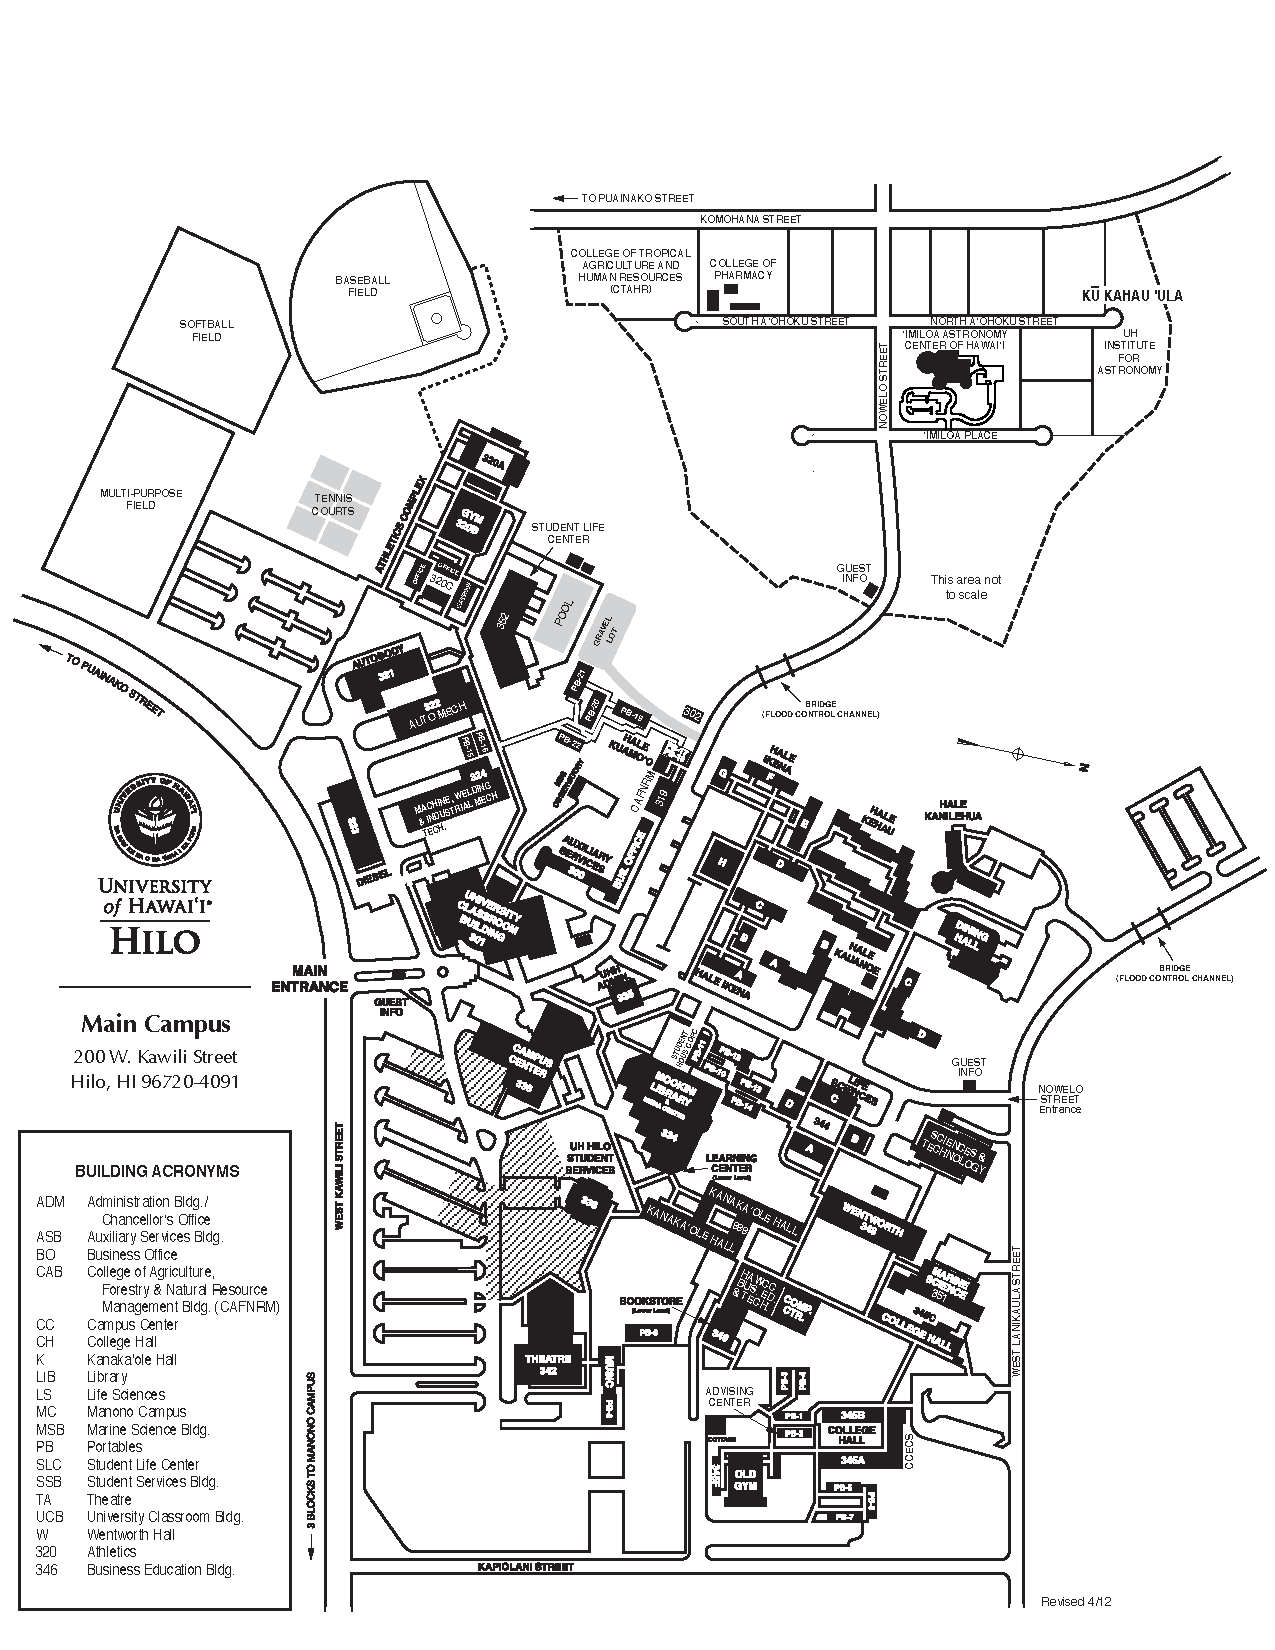
\includegraphics[scale=.25]{main_campus_map.pdf}| produces:

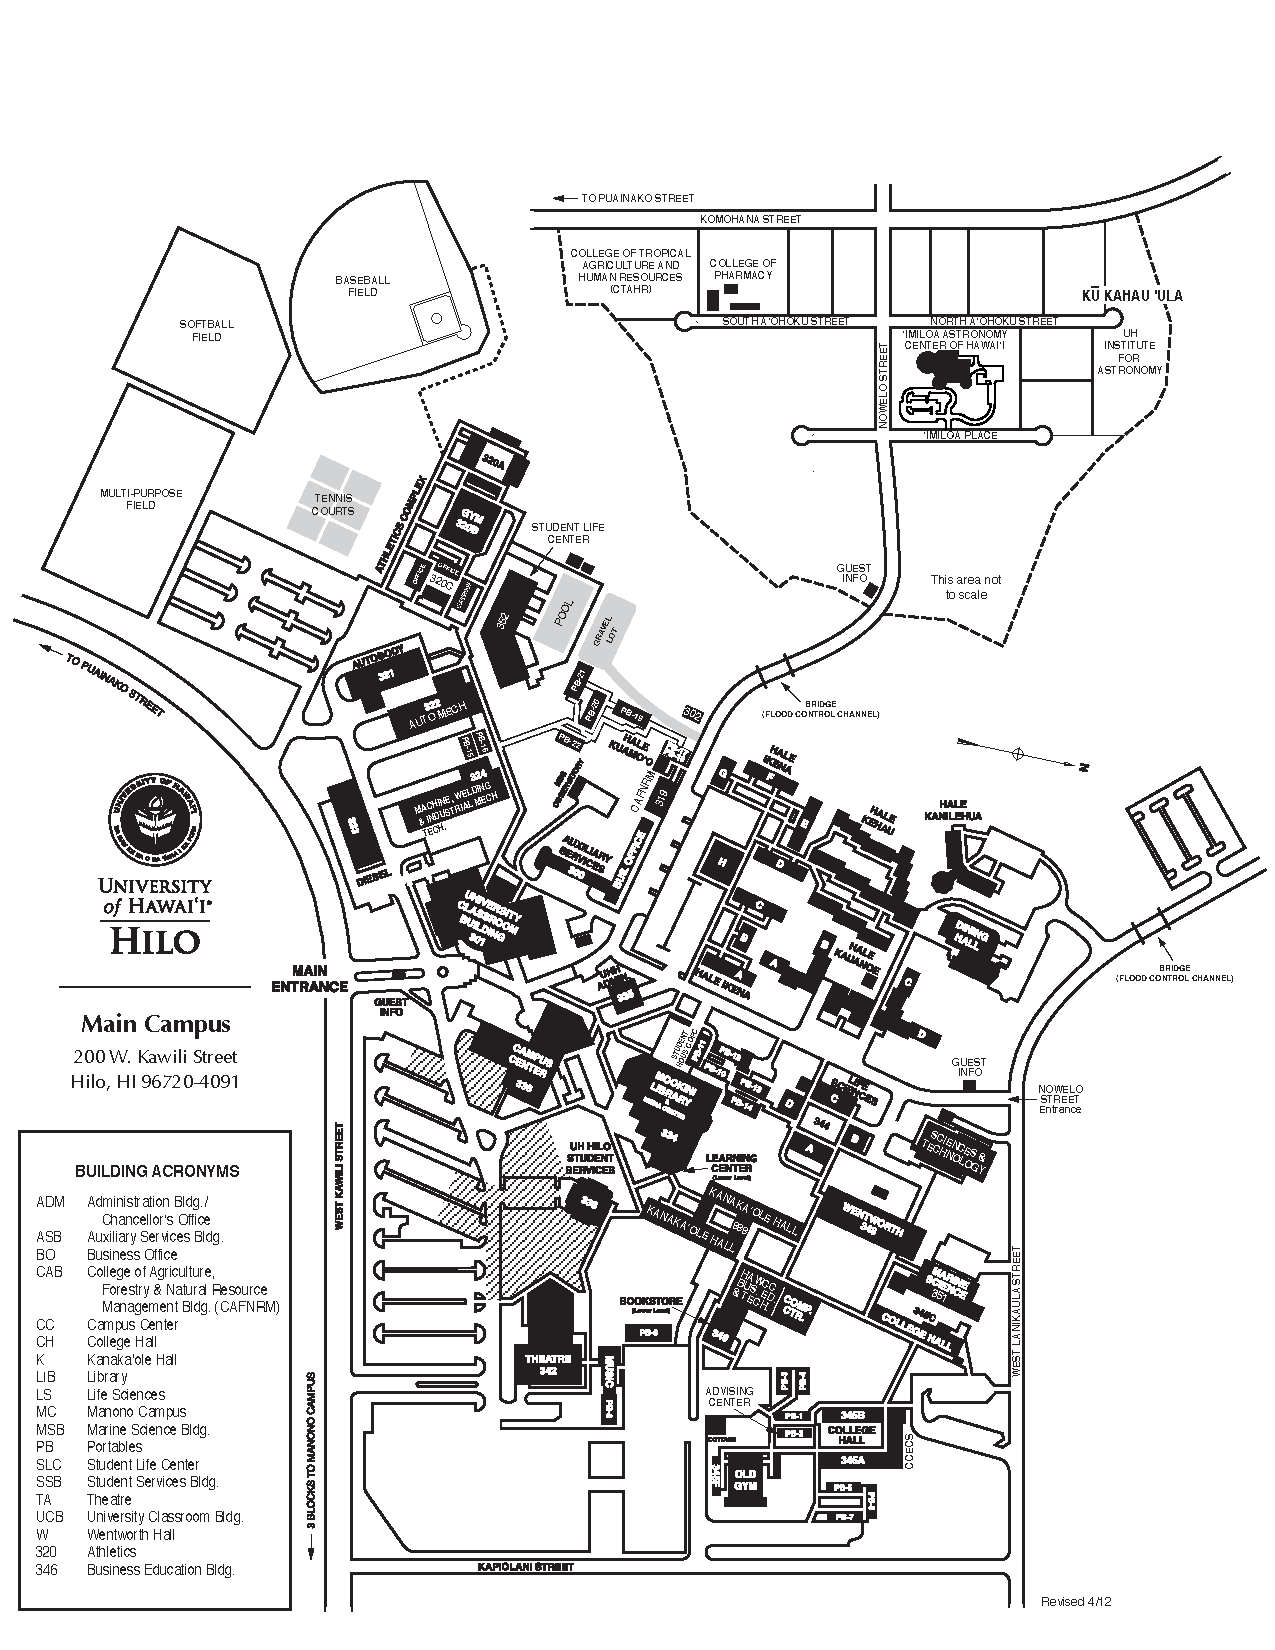
\includegraphics[scale=.25]{main_campus_map.pdf}

The graphics document must be in the same folder as your \LaTeX{} document. The graphics file may be .pdf, .png, or .jpg.

Notice how you can change the size using the ``scale'' option (in square brackets). Instead of specifying a scale factor, you can also choose the width or height (or both). For example, replace \verb|scale=.25| with \verb|width=1in| to get a picture 1 inch wide (the height will be automatically adjusted to keep the aspect ratio.

\subsection{Tables}

If you want to include a table, you use the \verb|tabular| environment. Here is a simple example.

\begin{verbatim}
\begin{tabular}{cc}
Name & Grade \\
John & 99 \\
Jane & 100 \\
\end{tabular}
\end{verbatim}

produces:

\begin{tabular}{cc}
Name & Grade \\
John & 99 \\
Jane & 100 \\
\end{tabular}

The \verb|{cc}| after the \verb|\begin{tabular}| specifies the number of columns, as well as the alignment. Two c's means you have two columns, and both are centered. If you want two columns that are right aligned, use \verb|{rr}|, and if you want them left aligned use \verb|{ll}|.

Here is an example with three columns, where the first is left aligned, the second is centered, and the third is right aligned:

\begin{verbatim}
\begin{tabular}{lcr}
Name & Exam Grade & Course Grade \\
John & 89 & B \\
Jane & 100 & A \\
\end{tabular}
\end{verbatim}

produces:

\begin{tabular}{lcr}
Name & Exam Grade & Course Grade \\
John & 89 & B \\
Jane & 100 & A \\
\end{tabular}

Notice that each row of the table has an ampersand (\verb|&|) between each column and a double backslash (\verb|\\|) at the end of the line.

If you want to add horizontal lines, you place \verb|\hline| between the rows.

\begin{verbatim}
\begin{tabular}{lcr}
Name & Exam Grade & Course Grade \\
\hline
John & 89 & B \\
Jane & 100 & A \\
\end{tabular}
\end{verbatim}

produces:

\begin{tabular}{lcr}
Name & Exam Grade & Course Grade \\
\hline
John & 89 & B \\
Jane & 100 & A \\
\end{tabular}

If you want to add vertical lines, you place a vertical bar ($|$) between the l, c, or r used to specify the number of columns.

\begin{verbatim}
\begin{tabular}{l|c|r}
Name & Exam Grade & Course Grade \\
\hline
John & 89 & B \\
Jane & 100 & A \\
\end{tabular}
\end{verbatim}

produces:

\begin{tabular}{l|c|r}
Name & Exam Grade & Course Grade \\
\hline
John & 89 & B \\
Jane & 100 & A \\
\end{tabular}

Here is a final example with lines everywhere:

\begin{verbatim}
\begin{tabular}{|l|c|r|}
\hline
Name & Exam Grade & Course Grade \\
\hline
John & 89 & B \\
\hline
Jane & 100 & A \\
\hline
\end{tabular}
\end{verbatim}

produces:

\begin{tabular}{|l|c|r|}
\hline
Name & Exam Grade & Course Grade \\
\hline
John & 89 & B \\
\hline
Jane & 100 & A \\
\hline
\end{tabular}

There are many more things you can do with tables, but these are the basics.

\section{Math in \LaTeX}

As we learned in Math 205, if we want to type math, we enclose the appropriate commands in dollar signs.

For example, type \verb|$f(x)=x^2+3x+2$| to get $f(x)=x^2+3x+2$.

Using single dollar signs produces typeset math inline. If you have math that you want set off from the rest of the text, enclose it in double dollar signs (display mode). For example, typing \verb|$$f(x)=x^2+3x+2$$| produces $$f(x)=x^2+3x+2$$

Note: If you have a long math formula on one line, you just have to put one set of dollar signs at the beginning and end of the line. You should not put dollar signs around each individual math command.

\subsection{Fractions}

To produce a fraction, type \verb|$\frac{numerator}{denominator}$|.

For example, typing \verb|$\frac{3}{7}$| produces $\frac{3}{7}$.

Typing \verb|$\frac{x^2+3x+9}{2x-4}$| produces $\frac{x^2+3x+9}{2x-4}$.

If these fractions are too small, you can make them larger by typing \verb|\ds| at the beginning:

Typing \verb|$\ds\frac{x^2+3x+9}{2x-4}$| produces $\ds\frac{x^2+3x+9}{2x-4}$.

Note that \verb|\ds| is not required when you use double dollar signs.

Typing \verb|$$\frac{x^2+3x+9}{2x-4}$$| produces $$\frac{x^2+3x+9}{2x-4}$$

\subsection{Powers and Roots}

If you have an exponent that is only one character, you can simply type a caret. For example, typing \verb|$x^2$| produces $x^2$.

If your exponent has more than one character (whether it's $-1$, $25$, or $x^2-3x+2$), enclose the exponent in curly brackets.

Compare what happens with \verb|$3^-2$| and \verb|$3^{-2}$|:

$3^-2$ versus $3^{-2}$ [in the first case, only the negative symbol is in the exponent]

Here's another example. To get $3^{x^2-8x+6}$ you type \verb|$3^{x^2-8x+6}$|.

To get a square root, use \verb|\sqrt{}|.

For example, \verb|$\sqrt{2}$| produces $\sqrt{2}$.

And \verb|$\sqrt{3x^2-5x+1}$| produces $\sqrt{3x^2-5x+1}$.

If you want a cube root, 4th root, etc., enclose the root number in square brackets after \verb|\sqrt|.

For example, \verb|$\sqrt[3]{2}$| produces $\sqrt[3]{2}$.

And \verb|$\sqrt[8]{\frac{3x+1}{9x+2}}$| produces $\sqrt[8]{\frac{3x+1}{9x+2}}$.

Or \verb|$\ds\sqrt[8]{\frac{3x+1}{9x+2}}$| produces $\displaystyle\sqrt[8]{\frac{3x+1}{9x+2}}$.

\subsection{Limits}

To display a limit symbol, you type \verb|\lim|. To get text below the limit symbol, use an underscore followed by curly brackets.

Here's an example:

\verb|$\lim_{x\to 1}f(x)$| produces $\lim_{x\to 1}f(x)$. [Notice that \verb|\to| produces the arrow.]

This usually looks better using \verb|\ds|:

\verb|$\ds\lim_{x\to 1}f(x)$| produces $\ds\lim_{x\to 1}f(x)$.

Here's another example:

\verb|$\ds\lim_{h\to 0}\frac{f(x+h)-f(x)}{h}$| produces $\ds\lim_{h\to 0}\frac{f(x+h)-f(x)}{h}$.

To get a limit at infinity, use \verb|\infty|:

Typing \verb|$\ds\lim_{x\to\infty}f(x)$| produces $\ds\lim_{x\to\infty}f(x)$.

or typing \verb|$\ds\lim_{x\to -\infty}f(x)$| produces $\ds\lim_{x\to -\infty}f(x)$.

For left and right limits, use the caret (\verb|^|) to put a plus or minus sign in the right spot:

For example, \verb|$\displaystyle\lim_{x\to 1^+}f(x)$| produces $\displaystyle\lim_{x\to 1^+}f(x)$.

And \verb|$\displaystyle\lim_{x\to 1^-}f(x)$| produces $\displaystyle\lim_{x\to 1^-}f(x)$.

\subsection{Derivatives}

Type \verb|$f'(x)$| to get $f'(x)$.

For the second derivative, type \verb|$f''(x)$| to get $f''(x)$.

For the third derivative, type \verb|$f'''(x)$| to get $f'''(x)$.

For higher order derivatives, use the caret (\verb|^|).

For example, \verb|$f^{(5)}(x)$| produces $f^{(5)}(x)$. [Don't forget the curly brackets around the exponent.]

If you want to use Leibniz's notation, you can type $\frac{d}{dx}$ just like a regular fraction.

For example, \verb|$\frac{d}{dx}f(x)$| produces $\frac{d}{dx}f(x)$.

Here is an example for the 3rd derivative: \verb|$\frac{d^3}{dx^3}f(x)$| produces $\frac{d^3}{dx^3}f(x)$.

\subsection{Summation Notation}

To get a summation symbol, type \verb|\sum|.

For example, \verb|$\sum i^2$| produces $\sum i^2$.

To add a range of values for the sum, use \verb|_| and \verb|^|.

For example, \verb|$\sum_{i=0}^{10} i^2$| produces $\sum_{i=0}^{10} i^2$. [Note the curly brackets around i=0 and 10.]

This will look better with \verb|\ds| or double dollar signs:

$\ds\sum_{i=0}^{10}i^2$ from \verb|$\displaystyle\sum_{i=0}^{10}i^2$|, or

$$\sum_{i=0}^{10}i^2$$ from \verb|$$\sum_{i=0}^{10}i^2$$|

\subsection{Integrals}

To get the integral symbol, type \verb|\int|.

For example, \verb|$\int f(x)$| produces $\int f(x)$.

If you want to add the $dx$, you should add an extra space by typing \verb|\,| before $dx$:

\verb|$\int f(x)\,dx$| produces $\int f(x)\,dx$. [Without \verb|\,| you get $\int f(x) dx$ - no space between $f(x)$ and $dx$]

Here's what you get if you add \verb|\ds|: $\ds\int f(x)\,dx$.

If you want a definite integral, you add a lower limit after an underscore and an upper limit after a caret.

For example, typing \verb|$\int_a^b f(x)\,dx$| produces $\int_a^b f(x)\,dx$.

Or, with \verb|\ds| you get $\ds\int_a^b f(x)\,dx$.

If a limit of integration is more than one character, then enclose it in curly brackets:

Typing \verb$\ds\int_{-2}^{18}f(x)\,dx$| produces $\ds\int_{-2}^{18} f(x)\, dx$.

Here's what the same integral looks like in display mode (double dollar signs): $$\int_{-2}^{18} f(x)\, dx$$

\subsection{Miscellaneous Symbols}

To get ``approximately equal to,'' use \verb|\approx|. For example, \verb|$x\approx 20$| produces $x\approx20$.

To get the plus or minus symbol, use \verb|\pm|. For example, \verb|$\pm 3$| produces $\pm3$.

To get a Greek letter, type a backslash and write out the name of the letter. For example, \verb|$\pi$| produces $\pi$ and \verb|$\alpha$| produces $\alpha$.

For the capital Greek letters, capitalize the first letter: \verb|$\Pi$| produces $\Pi$ and \verb|$\Sigma$| produces $\Sigma$.

[Note: If the capital Greek letter is the same as the Latin capital, then the Greek won't work. For example, \verb|$\Alpha$| will produce an error, since capital alpha is $A$.]

To get $\ge$ and $\le$, type \verb|$\ge$| or \verb|$\le$|. To get \verb|<| or \verb|>|, simply use the keyboard.

For multiplication, you can use either \verb|\times| or \verb|\cdot|. For example, \verb|$x\times y$| prodcues $x\times y$ and \verb|$x\cdot y$| produces $x\cdot y$.

For composition of functions, use \verb|\circ|. For example, \verb|$f\circ g$| produces $f\circ g$.

For an ellipsis (three dots), use either \verb|\dots| or \verb|\cdots|. The former has three dots along the base line, while the latter has three dots centered vertically. Here is an example of each:

\verb|$1,\ 2,\ 3,\ \dots$| produces $1,\ 2,\ 3,\ \dots$

\verb|$1+2+3+\cdots$| produces $1+2+3+\cdots$

The \verb|\cancel| command can be used to cross things out (this requires the cancel package). For example:

\begin{verbatim}
$$\frac{(x+1)\cancel{(x+2)}}{(x-3)\cancel{(x+2)}}=\frac{x+1}{x-3}$$
\end{verbatim}

produces

$$\frac{(x+1)\cancel{(x+2)}}{(x-3)\cancel{(x+2)}}=\frac{x+1}{x-3}$$

There is also a \verb|\cancelto| command to do things like this:

$$\lim_{x\to \infty}\frac{2+\cancelto{0}{\frac{3}{x}}-\cancelto{0}{\frac{2}{x^2}}}{3-\cancelto{0}{\frac{1}{x}}+\cancelto{0}{\frac{4}{x^2}}}=\frac{2}{3}$$

Here is the code:

\begin{verbatim}
$$\lim_{x\to \infty}\frac{2+\cancelto{0}{\frac{3}{x}}
-\cancelto{0}{\frac{2}{x^2}}}{3-\cancelto{0}{\frac{1}{x}}
+\cancelto{0}{\frac{4}{x^2}}}=\frac{2}{3}$$
\end{verbatim}

Notice that \verb|\cancelto| requires two arguments, a value and an expression. For example, \verb|\cancelto{10}{x}| produces $\cancelto{10}{x}$.

For more symbols, refer to the PDF ``LaTeX Symbol List.''

\subsection{Re-sizing Parentheses}

If you put regular-sized parentheses around a tall mathematical expression, it will not look right. For example, $\ds f(\frac{3x+2}{9x-1})$ would look better with larger parentheses, like this $\ds f\left(\frac{3x+2}{9x-1}\right)$.

To do this in \LaTeX{} you use the \verb|\left| and \verb|\right| commands. You place \verb|\left| in front of the left parenthesis and \verb|\right| in front of the right one. This also works for square brackets, curly brackets, and vertical bars. Here are examples of each.

\begin{itemize}

\item \begin{verbatim}$\ds\left(\frac{4x^2}{9x^5}\right)$\end{verbatim}

produces $\ds\left(\frac{4x^2}{9x^5}\right)$

\item \begin{verbatim}$\ds\left[\frac{4x^2}{9x^5}\right]$\end{verbatim}

produces $\ds\left[\frac{4x^2}{9x^5}\right]$

\item \begin{verbatim}$\ds\left\{\frac{4x^2}{9x^5}\right\}$\end{verbatim}

produces $\ds\left\{\frac{4x^2}{9x^5}\right\}$

[Notice the \verb|\{| and \verb|\}| to get curly brackets.]

\item \begin{verbatim}$\ds\left|\frac{4x^2}{9x^5}\right|$\end{verbatim}

produces $\ds\left|\frac{4x^2}{9x^5}\right|$

\end{itemize}

Every \verb|\left| must be paired with a \verb|\right|, and vice versa, but the symbol does not have to be the same thing. For example,

\begin{verbatim}$\ds\left(\frac{4x^2}{9x^5}\right]$\end{verbatim}

produces $\ds\left(\frac{4x^2}{9x^5}\right]$

If you want a parenthesis, etc. on only one side, then you put a period (.) on the other side (since left and right must be matched, even if you don't want anything on one side). For example,

\begin{verbatim}$\ds\left.\frac{4x^2}{9x^5}\right|_{x=2}$\end{verbatim}

produces $\ds\left.\frac{4x^2}{9x^5}\right|_{x=2}$

[Notice \verb|\left.| does not produce a period, it's merely a placeholder. The height of everything between \verb|\left| and \verb|\right| determines the height of the parenthesis, etc., so both need to be there.]

\subsection{Text in Math Mode}

If you put text within dollar signs, all spaces are ignored and everything is placed in italics.

To avoid this, use \verb|\text|. Compare the following:

\verb|$f(x) and g(x)$| produces $f(x) and g(x)$

\verb|$f(x) \text{ and } g(x)$| produces $f(x) \text{ and } g(x)$ [Notice the spaces around "and"]

\subsection{Getting \LaTeX{} Code from Sage}

If you have a mathematical expression in Sage, you can convert it to \LaTeX{} code using the \texttt{latex(...)} command.

For example, in a Sage worksheet type latex(3/4) and hit ``Run.'' The output will be \verb|\frac{3}{4}|.

Or suppose you run \verb|derivative(cos(1/x^5))| in a Sage worksheet, which produces the output \verb|5*sin(x^(-5))/x^6|. If you want to convert this answer to \LaTeX{}, simply type \verb|latex(_)| in the next cell and hit ``Run'' [remember, \verb|_| recalls the last output; you could also copy and paste to do \verb|latex(5*sin(x^(-5))/x^6)|]. Then Sage produces the output \verb|\frac{5 \, \sin\left(\frac{1}{x^{5}}\right)}{x^{6}}|

[You may notice that the \LaTeX{} code produced by Sage is more complicated than your own, but it shouldn't be a problem.]

\section{Using Sage in \LaTeX}

Sometimes we want to use the result of a calculation in a \LaTeX{} document. One way to do this would be to perform the calculation elsewhere and then copy the answer into our document. However, using the sagetex package (which I have included), we can get Sage to output results directly into \LaTeX{}.

\subsection{Getting Output from Sage}

To perform a calculation in Sage and get the output in your \LaTeX{} document, use the \verb|\sage| command. Here are some examples:

\begin{itemize}

\item Typing \verb|$\sage{2+2}$| produces $\sage{2+2}$.

\item Typing \verb|$\sage{2^3*3^4*5^2}$| produces $\sage{2^3*3^4*5^2}$.

\item Typing \verb|$\sage{derivative(sin(x^2),x)}$| produces $\sage{derivative(sin(x^2),x)}$.

\end{itemize}

Since Sage output often includes mathematical symbols, you should usually put dollar signs around \verb|\sage{...}|.

\subsection{Graphing}

You can plot graphs using the \verb|\sageplot| command. It is similar to \verb|\includegraphics| (see section \ref{ingr} above). You can specify either a scale factor or the width or height directly. For example, \verb|\sageplot[width=1in]{plot(x^2)}| produces:

\sageplot[width=1in]{plot(x^2)}

Within the parentheses after \verb|plot| you can include all the options you would normally use in Sage. For example,

\verb|\sageplot[height=2in]{plot(cos(x),xmin=-pi,xmax=pi,color='salmon')}|

produces:

\sageplot[height=2in]{plot(cos(x),xmin=-pi,xmax=pi,color='salmon')}

\subsection{Sending Input to Sage}

If you want to send things to Sage, you have two options, the \verb|sageblock| and \verb|sagesilent| environments. When you use \verb|sageblock|, the Sage code itself is typeset in your \LaTeX{} output, and the code is run in Sage. When you use \verb|sagesilent|, the Sage code is \emph{not} typeset, it is only run in Sage. For example,

\begin{verbatim}
\begin{sageblock}
f(x)=3*x+2
g(x)=4*x^2
h(x)=derivative(f*g,x)
\end{sageblock}
\end{verbatim}
produces this output:

\begin{sageblock}
f(x)=3*x+2
g(x)=4*x^2
h(x)=derivative(f*g,x)
\end{sageblock}

These three functions are now available in Sage. For example, if I want $h(2)$ I can type \verb|$\sage{h(2)}$| in the \LaTeX{} file, and I will get $\sage{h(2)}$.

Once I have defined a variable or function using \verb|sageblock| (or \verb|sagesilent|), I can use it again anywhere in my document. For example, I will now define a new function $k$ to be the integral of the $g$ function. I will type the following:

\begin{verbatim}
\begin{sagesilent}
k(x)=integrate(g,x)
\end{sagesilent}
\end{verbatim}

This Sage block will not appear in my \LaTeX{} output (I have manually included it here).

\begin{sagesilent}
k(x)=integrate(g,x)
\end{sagesilent}

The $k$ function can now be used. So here is $k(4)$: $\sage{k(4)}$ (type \verb|$\sage{k(4)}$|).

Note: Use \verb|sageblock| and \verb|sagesilent| to \emph{input} things into Sage. These do \emph{not} bring the Sage output into your \LaTeX{} document. To get Sage output to appear, use \verb|\sage{...}|.

\subsection{Problems with Sage in \LaTeX{}}

Sometimes the Sage commands you run in \LaTeX{} do not produce the desired output. This can happen because Sage runs too slowly, so \LaTeX{} gives up on it and continues processing. This can result in ``??" showing up in the output, or the incorrect output may appear.

When this happens, you can usually fix it manually:

\begin{enumerate}

\item Click on the ``Build" tab in the output pane.

\item Click on the ``Sage" button. You may have to wait a little while for this to finish.

\item Click on the ``Latex" button. Again, it may take some time to process.

\item Finally, return to the ``Preview." It may take 20 or 30 seconds for the preview to update, but most of the time it will.

\end{enumerate}

Another possibility is that you have an error in your Sage code, so Sage is not producing the expected output. If the above steps do not help, double-check your Sage code. If necessary, you may have to copy your code to a Sage worksheet and check for errors there.

\section{You're Ready to Go}

I have included a \LaTeX{} template document in this assignment folder. When you want to create your own \LaTeX{} document, I suggest the following:

\begin{enumerate}

\item Create a new folder for your \LaTeX{} document (several auxiliary files will be created, and you don't want to clutter up your home directory).

\item Copy the template file (LaTeX Template.tex) into this new folder (click the check box next to the file, press the ``Copy" button near the top of the page, select the new folder from the drop-down menu under ``Destination," and click the blue ``Copy" button).

\item Open the new folder, click the check box next to the template, and click the ``Rename" button near the top of the page. Change the name as desired and click the blue ``Rename item" button.

\item Now open this \LaTeX{} file and you're ready to begin.

\end{enumerate}

Remember to leave the original template blank for future use.

You will be using \LaTeX{} for your assignment today. Open the file ``Writing in LaTeX Assignment.tex" for instructions.

Also note that your group assignment will be written entirely in \LaTeX{}, and you will be submitting a hard copy in two weeks.

\section{If You Need More Help}

There is a large community of \LaTeX{} users online, so a simple search will answer many of your questions. For example if you google ``latex table," you can find instructions for producing tables from many different sources.

There is a series of brief videos on YouTube about using \LaTeX{} in CoCalc (these videos refer to SageMathCloud, the former name of CoCalc) available here:

{\color{blue}\underline{\url{https://www.youtube.com/playlist?list=PLnC5h3PY-znxc090kGv7W4FpbotlWsrm0}}}

[This should be an active link in the PDF, but links don't work in the Preview.]

\section{License}

This material was developed by Aaron Tresham at the University of Hawaii at Hilo and is licensed under a \href{http://creativecommons.org/licenses/by-sa/4.0/}{\color{blue}\underline{Creative Commons Attribution-ShareAlike 4.0 International License.}}

\end{document}
